\documentclass[aspectratio=169,10pt]{beamer}
\usetheme{Madrid}
\usecolortheme{default}

\usepackage[utf8]{inputenc}
\usepackage[T1]{fontenc}
\usepackage[brazilian]{babel}
\usepackage{booktabs}
\usepackage{amsmath}
\usepackage{graphicx}
\usepackage{xspace}

% Números gerados por paper/gera_tabelas.py a partir de results/.
% Gerado por paper/gera_tabelas.py. Não editar à mão.
\newcommand{\NumMatrizes}{8\xspace}
\newcommand{\NumExecSpmv}{96\xspace}
\newcommand{\NumBitExatas}{96\xspace}
\newcommand{\MinLinhas}{30\xspace}
\newcommand{\MaxLinhas}{1033\xspace}
\newcommand{\MaxNnz}{6027\xspace}
\newcommand{\MedFPtrinta}{$5.91 \times 10^{-8}$\xspace}
\newcommand{\MedTakumTrinta}{$1.15 \times 10^{-8}$\xspace}
\newcommand{\MedFPtrintaAcSes}{$3.61 \times 10^{-8}$\xspace}
\newcommand{\MedTakumTrintaAcTrinta}{$2.94 \times 10^{-8}$\xspace}
\newcommand{\MedTakumTrintaScaled}{$5.37 \times 10^{-9}$\xspace}
\newcommand{\MedBF}{$2.36 \times 10^{-3}$\xspace}
\newcommand{\MedTakumDez}{$7.43 \times 10^{-4}$\xspace}
\newcommand{\MedTakumDezScaled}{$3.09 \times 10^{-4}$\xspace}
\newcommand{\MedTakumOito}{$1.52 \times 10^{-1}$\xspace}
\newcommand{\MedTakumOitoScaled}{$8.39 \times 10^{-2}$\xspace}
\newcommand{\RazaoFormatoAcTrinta}{2.01\xspace}
\newcommand{\RazaoAcumuladorTakum}{2.56\xspace}
\newcommand{\RazaoKernelTrinta}{5.15\xspace}
\newcommand{\RazaoAcAmpliadoTrinta}{3.15\xspace}
\newcommand{\RazaoTakumBF}{3.17\xspace}
\newcommand{\RazaoTakumBFScaled}{7.61\xspace}
\newcommand{\ParTrintaFPAmbos}{8\xspace}
\newcommand{\ParTrintaFPTakumVence}{7\xspace}
\newcommand{\ParTrintaFPOutroVence}{1\xspace}
\newcommand{\ParTrintaFPEmpates}{0\xspace}
\newcommand{\ParTrintaFPTakumNF}{0\xspace}
\newcommand{\ParTrintaFPOutroNF}{0\xspace}
\newcommand{\ParTrintaAcFPAmbos}{8\xspace}
\newcommand{\ParTrintaAcFPTakumVence}{7\xspace}
\newcommand{\ParTrintaAcFPOutroVence}{1\xspace}
\newcommand{\ParTrintaAcFPEmpates}{0\xspace}
\newcommand{\ParTrintaAcFPTakumNF}{0\xspace}
\newcommand{\ParTrintaAcFPOutroNF}{0\xspace}
\newcommand{\ParDezFPAmbos}{5\xspace}
\newcommand{\ParDezFPTakumVence}{3\xspace}
\newcommand{\ParDezFPOutroVence}{2\xspace}
\newcommand{\ParDezFPEmpates}{0\xspace}
\newcommand{\ParDezFPTakumNF}{0\xspace}
\newcommand{\ParDezFPOutroNF}{3\xspace}
\newcommand{\ParDezBFAmbos}{8\xspace}
\newcommand{\ParDezBFTakumVence}{7\xspace}
\newcommand{\ParDezBFOutroVence}{1\xspace}
\newcommand{\ParDezBFEmpates}{0\xspace}
\newcommand{\ParDezBFTakumNF}{0\xspace}
\newcommand{\ParDezBFOutroNF}{0\xspace}
\newcommand{\ParOitoEquatromAmbos}{4\xspace}
\newcommand{\ParOitoEquatromTakumVence}{0\xspace}
\newcommand{\ParOitoEquatromOutroVence}{4\xspace}
\newcommand{\ParOitoEquatromEmpates}{0\xspace}
\newcommand{\ParOitoEquatromTakumNF}{0\xspace}
\newcommand{\ParOitoEquatromOutroNF}{4\xspace}
\newcommand{\ParOitoCincodoisAmbos}{5\xspace}
\newcommand{\ParOitoCincodoisTakumVence}{3\xspace}
\newcommand{\ParOitoCincodoisOutroVence}{2\xspace}
\newcommand{\ParOitoCincodoisEmpates}{0\xspace}
\newcommand{\ParOitoCincodoisTakumNF}{0\xspace}
\newcommand{\ParOitoCincodoisOutroNF}{3\xspace}
\newcommand{\NFTakumOito}{0\xspace}
\newcommand{\NFTakumDez}{0\xspace}
\newcommand{\NFEquatrom}{4\xspace}
\newcommand{\NFCincodois}{3\xspace}
\newcommand{\NFDez}{3\xspace}
\newcommand{\NFBF}{0\xspace}
\newcommand{\ElemNnzFP}{5.33\xspace}
\newcommand{\ElemNnzTakum}{4.50\xspace}
\newcommand{\InsnNnzFPCento}{6.14\xspace}
\newcommand{\CsrNnzFPCento}{1.33\xspace}
\newcommand{\InsnNnzFPDuzentos}{4.59\xspace}
\newcommand{\CsrNnzFPDuzentos}{1.07\xspace}
\newcommand{\InsnNnzFPQuinhentos}{4.34\xspace}
\newcommand{\CsrNnzFPQuinhentos}{1.03\xspace}
\newcommand{\InsnNnzTrintaCento}{5.98\xspace}
\newcommand{\CsrNnzTrintaCento}{1.33\xspace}
\newcommand{\RelInsnTrintaCento}{$-$2.7\%\xspace}
\newcommand{\RelCsrTrintaCento}{+0.0\%\xspace}
\newcommand{\EconomiaCento}{2.7\%\xspace}
\newcommand{\ZvtNnzTrintaCento}{0.50\xspace}
\newcommand{\InsnNnzTrintaDuzentos}{4.55\xspace}
\newcommand{\CsrNnzTrintaDuzentos}{1.07\xspace}
\newcommand{\RelInsnTrintaDuzentos}{$-$0.7\%\xspace}
\newcommand{\RelCsrTrintaDuzentos}{+0.0\%\xspace}
\newcommand{\EconomiaDuzentos}{0.7\%\xspace}
\newcommand{\ZvtNnzTrintaDuzentos}{0.37\xspace}
\newcommand{\InsnNnzTrintaQuinhentos}{4.33\xspace}
\newcommand{\CsrNnzTrintaQuinhentos}{1.03\xspace}
\newcommand{\RelInsnTrintaQuinhentos}{$-$0.3\%\xspace}
\newcommand{\RelCsrTrintaQuinhentos}{+0.0\%\xspace}
\newcommand{\EconomiaQuinhentos}{0.3\%\xspace}
\newcommand{\ZvtNnzTrintaQuinhentos}{0.35\xspace}
\newcommand{\InsnNnzDezCento}{4.95\xspace}
\newcommand{\CsrNnzDezCento}{1.47\xspace}
\newcommand{\RelInsnDezCento}{$-$19.3\%\xspace}
\newcommand{\RelCsrDezCento}{+10.7\%\xspace}
\newcommand{\ZvtNnzDezCento}{0.37\xspace}
\newcommand{\InsnNnzDezDuzentos}{4.69\xspace}
\newcommand{\CsrNnzDezDuzentos}{1.39\xspace}
\newcommand{\RelInsnDezDuzentos}{+2.2\%\xspace}
\newcommand{\RelCsrDezDuzentos}{+29.9\%\xspace}
\newcommand{\ZvtNnzDezDuzentos}{0.35\xspace}
\newcommand{\InsnNnzDezQuinhentos}{4.60\xspace}
\newcommand{\CsrNnzDezQuinhentos}{1.36\xspace}
\newcommand{\RelInsnDezQuinhentos}{+6.0\%\xspace}
\newcommand{\RelCsrDezQuinhentos}{+32.5\%\xspace}
\newcommand{\ZvtNnzDezQuinhentos}{0.34\xspace}
\newcommand{\InsnNnzOitoCento}{4.51\xspace}
\newcommand{\CsrNnzOitoCento}{1.39\xspace}
\newcommand{\RelInsnOitoCento}{$-$26.6\%\xspace}
\newcommand{\RelCsrOitoCento}{+4.6\%\xspace}
\newcommand{\ZvtNnzOitoCento}{0.35\xspace}
\newcommand{\InsnNnzOitoDuzentos}{4.43\xspace}
\newcommand{\CsrNnzOitoDuzentos}{1.36\xspace}
\newcommand{\RelInsnOitoDuzentos}{$-$3.4\%\xspace}
\newcommand{\RelCsrOitoDuzentos}{+27.4\%\xspace}
\newcommand{\ZvtNnzOitoDuzentos}{0.34\xspace}
\newcommand{\InsnNnzOitoQuinhentos}{4.39\xspace}
\newcommand{\CsrNnzOitoQuinhentos}{1.35\xspace}
\newcommand{\RelInsnOitoQuinhentos}{+1.1\%\xspace}
\newcommand{\RelCsrOitoQuinhentos}{+31.2\%\xspace}
\newcommand{\ZvtNnzOitoQuinhentos}{0.34\xspace}
\newcommand{\InsnMenorTrinta}{13\xspace}
\newcommand{\InsnIgualTrinta}{11\xspace}
\newcommand{\InsnMaiorTrinta}{0\xspace}
\newcommand{\InsnMenorDez}{11\xspace}
\newcommand{\InsnIgualDez}{0\xspace}
\newcommand{\InsnMaiorDez}{13\xspace}
\newcommand{\InsnMenorOito}{12\xspace}
\newcommand{\InsnIgualOito}{0\xspace}
\newcommand{\InsnMaiorOito}{12\xspace}
\newcommand{\InsnPares}{24\xspace}
\newcommand{\ModRFP}{13\xspace}
\newcommand{\ModCFP}{12\xspace}
\newcommand{\ModKFP}{21\xspace}
\newcommand{\ModROito}{14\xspace}
\newcommand{\ModCOito}{12\xspace}
\newcommand{\ModKOito}{21\xspace}
\newcommand{\ModRDez}{14\xspace}
\newcommand{\ModCDez}{13\xspace}
\newcommand{\ModKDez}{21\xspace}
\newcommand{\ModRTrinta}{14\xspace}
\newcommand{\ModCTrinta}{11\xspace}
\newcommand{\ModKTrinta}{21\xspace}
\newcommand{\ModExatas}{96\xspace}
\newcommand{\ModExec}{96\xspace}
\newcommand{\ModSinteticosOk}{12\xspace}
\newcommand{\ModSinteticosTotal}{12\xspace}
\newcommand{\ModResiduoMax}{0\xspace}


\title[Takum na RVV (Zvtakum)]{Aritmética Takum na Extensão Vetorial RISC-V (Zvtakum)}
\subtitle{Projeto Integrador AOC/UFMG --- Entrega Final}
\author[Rezende, Fontes, Lopes, Brito]{André Luís Alves Rezende \and Gabriel Ramos Fontes \and Isadora Maria Carvalho Lopes \and João Pedro Santos de Brito}
\institute[DELT/UFMG]{Departamento de Engenharia Eletrônica (DELT) -- UFMG}
\date[2026]{2026}

\begin{document}

\begin{frame}
	\titlepage
\end{frame}

\begin{frame}{Motivação: proliferação de formatos na RVV}
	\begin{itemize}
		\item RVV hoje: FP16 (\texttt{Zvfh}), bfloat16
		      (\texttt{Zvfbfmin}/\texttt{Zvfbfwma}), FP32/64, cripto (\texttt{Zvk*}).
		      \textbf{FP8 não existe} na RVV~1.0.
		\item Cada subformato novo adiciona conversões cruzadas ($O(N^2)$), subnormais,
		      múltiplos NaNs e dependências em \texttt{fcsr} (\texttt{frm}/\texttt{fflags}).
		\item A \textbf{aritmética Takum} oferece precisão afilada (\emph{tapered precision}),
		      faixa dinâmica limitada ($\approx 10^{\pm 77}$) e \textbf{um decodificador comum de 12~MSBs}
		      para qualquer largura.
		\item Estendemos à RVV~1.0 a metodologia de consolidação de Hunhold para o
		      Intel AVX10.2 (MOCAST 2025): $92 + 4 = 96 \to 8$ primitivas aritméticas.
	\end{itemize}
\end{frame}

\begin{frame}{Codificação Takum Linear (Def. 8) e Precisão Afilada}
	\begin{itemize}
		\item Campos $(S, D, R, C, F)$: prefixo $(S,D,R,C)$ cabe sempre nos \textbf{12~MSBs} ($r \le 7$); \texttt{T8} recebe 4 \emph{ghost bits} nulos à direita.
		\item Complemento de dois monotônico; especiais únicos $0$ e \texttt{NaR}; saturação em $[\mathrm{minpos},\mathrm{maxpos}]$ sem infinito; \textbf{RNE no espaço de códigos}.
	\end{itemize}
	\centering
	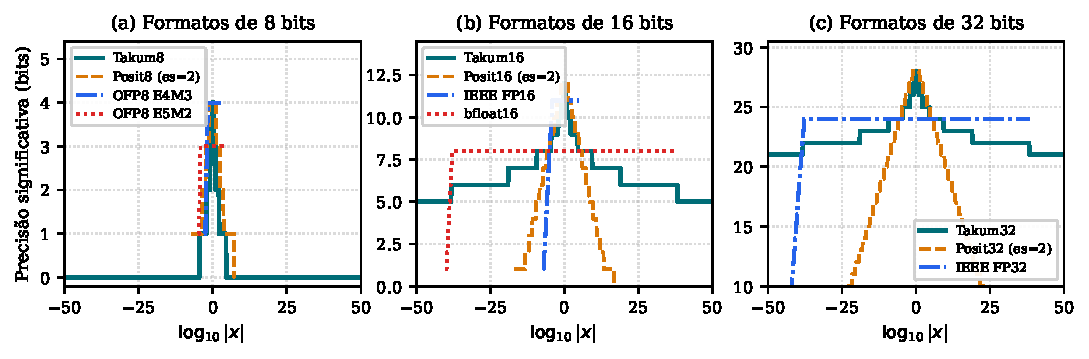
\includegraphics[width=0.90\textwidth]{../paper/figures/tapered-precision-pt.pdf}
\end{frame}

\begin{frame}{Extensão Zvtakum: cinco instruções em \texttt{custom-0}}
	\begin{table}
		\centering
		\footnotesize
		\begin{tabular}{llll}
			\toprule
			Mnemônico & \texttt{funct6} & Operação & Observação \\
			\midrule
			\texttt{vtadd.vv} & \texttt{000000} & $vd_i = vs2_i + vs1_i$ & RNE saturante (\texttt{SEW}) \\
			\texttt{vtsub.vv} & \texttt{000001} & $vd_i = vs2_i - vs1_i$ & RNE saturante (\texttt{SEW}) \\
			\texttt{vtmul.vv} & \texttt{000010} & $vd_i = vs2_i \times vs1_i$ & RNE saturante (\texttt{SEW}) \\
			\texttt{vtdot.vv} & \texttt{000011} & $vd_0 \leftarrow vd_0 + \sum_i vs2_i \cdot vs1_i$
			                  & acúmulo $2\cdot\mathrm{SEW}$ (\texttt{T16/T32/T64}) \\
			\texttt{vncvt.t.t} & \texttt{000100} & $T_{2\cdot\mathrm{SEW}} \to T_{\mathrm{SEW}}$ & estreitamento RNE (\texttt{vs1=0}) \\
			\bottomrule
		\end{tabular}
	\end{table}
	\begin{itemize}
		\item \texttt{opcode = 0x0B} (\texttt{custom-0}), \texttt{funct3 = 000}, \texttt{vm} no bit 25: preserva \texttt{OP-V} intacto.
		\item \texttt{vtype.vsew} seleciona \texttt{T8/T16/T32}; obedece a \texttt{vl}, \texttt{vstart}, \texttt{v0.t}, \texttt{vta}/\texttt{vma}; \textbf{zero dependência de \texttt{fcsr}}.
	\end{itemize}
\end{frame}

\begin{frame}{Caminho de Dados Proposto: RISC-V + Subsistema Zvtakum}
	\centering
	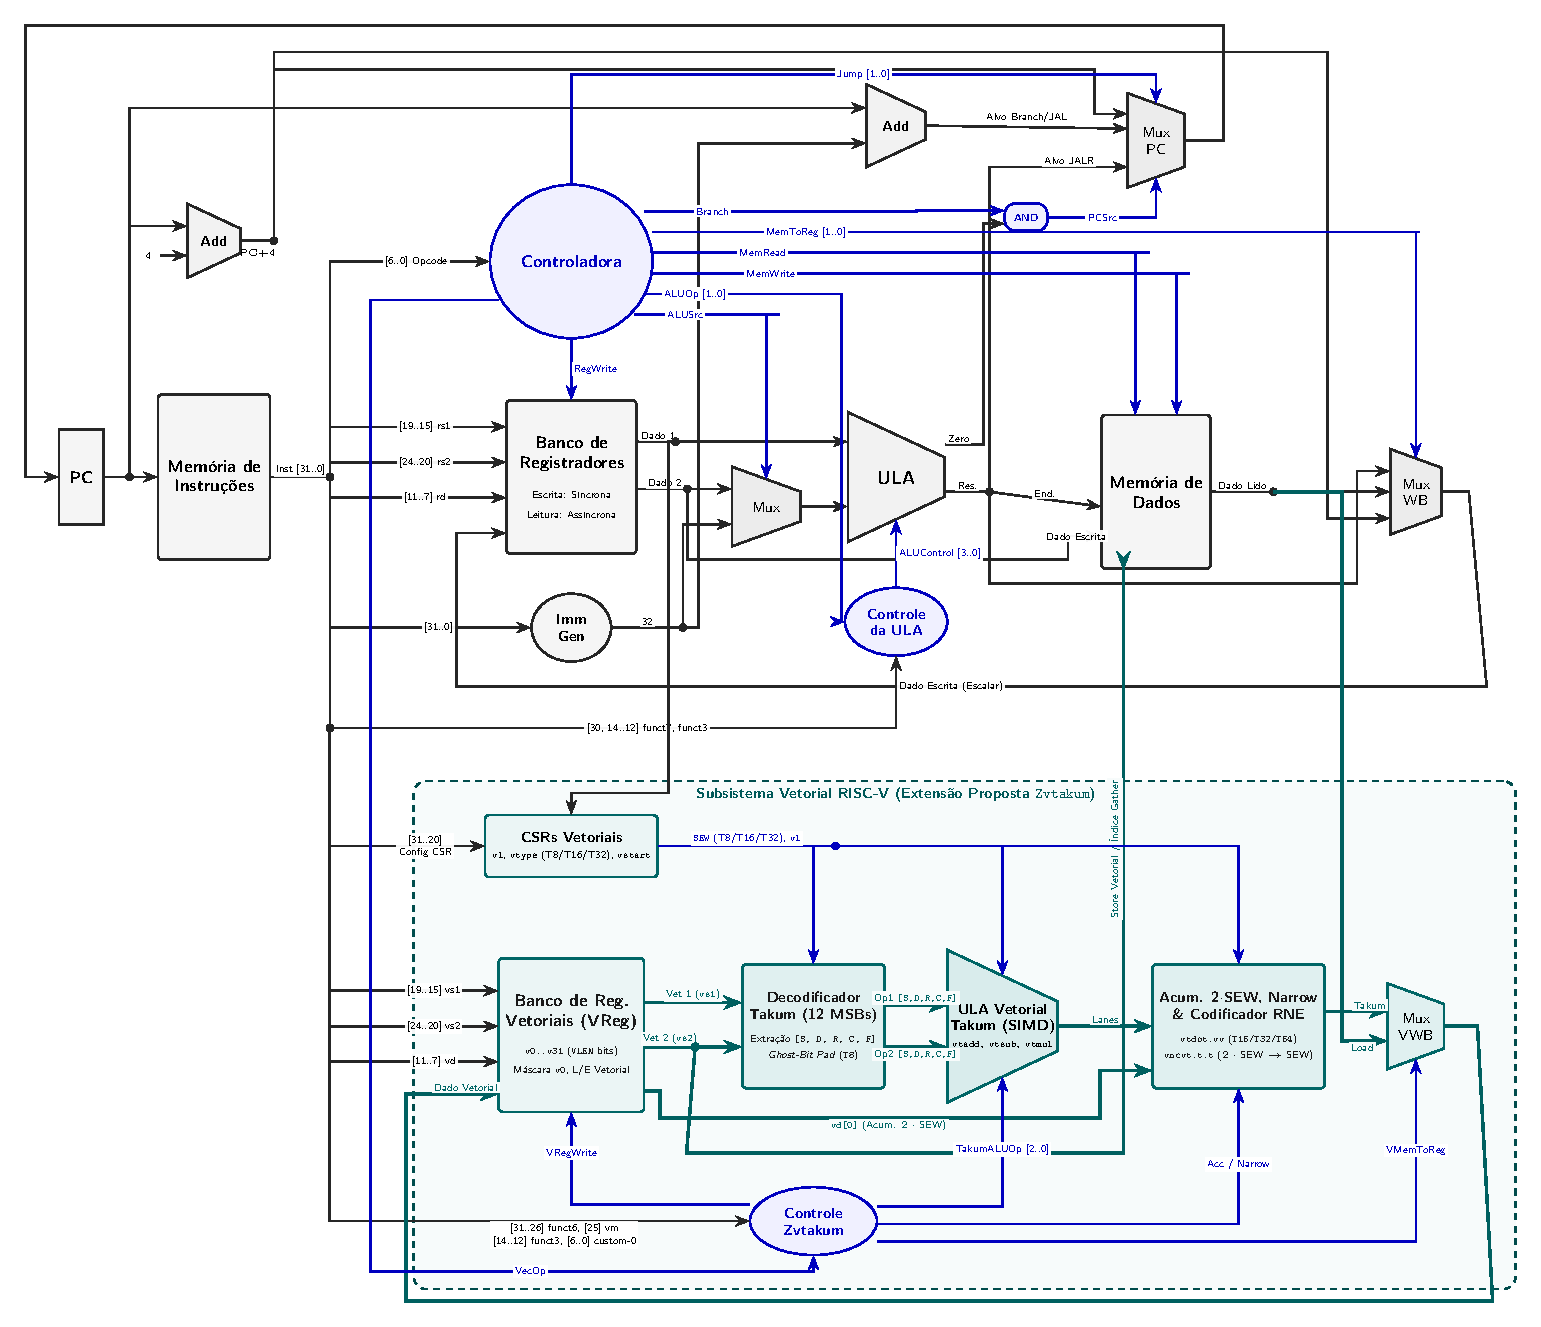
\includegraphics[height=0.76\textheight]{../paper/figures/datapath_zvtakum_pt.pdf}
\end{frame}

\begin{frame}{ULA Takum em Inteiros de 128 Bits e Simulador \texttt{zt-sim}}
	\begin{itemize}
		\item \textbf{Sem \texttt{double} do hospedeiro:} \texttt{src/takum.cpp} usa apenas \texttt{uint64\_t} e \texttt{unsigned \_\_int128} para tupla exata $(-1)^{\mathrm{neg}}\cdot\mathrm{sig}\cdot 2^{e-63}$.
		\item \textbf{Descoberta de duplo arredondamento:} 0 divergências contra \texttt{libtakum} v2.0.0 em 196.608 pares \texttt{T8} e 50.000 \texttt{T16}; em \texttt{T32}, 128/30.000 produtos no limiar de empate diferem por 1~ULP devido ao intermediário \texttt{double} da \texttt{libtakum}.
		\item \textbf{Oráculo \texttt{binary128}:} validado em 6.017 testes contra \texttt{\_\_float128}/\texttt{libquadmath} (GCC 9.4.0).
		\item \textbf{Verificação diferencial:} \texttt{zt-sim} coincide byte a byte com \texttt{qemu-riscv64}~10.2.2 em $\mathrm{VLEN}\in\{128,256,512\}$ (9 execuções, 0 divergências) e em todas as \NumExecSpmv\ execuções SpMV.
	\end{itemize}
\end{frame}

\begin{frame}{Resultado 1: Acurácia SpMV em 32 Bits e Papel do Acumulador}
	\begin{itemize}
		\item Kernel RVV \texttt{FP32} (ac.\ 32b): mediana \MedFPtrinta; \texttt{Takum32} (\texttt{vtdot} ac.\ 64b): \MedTakumTrinta\ ($\RazaoKernelTrinta\times$ menor erro, vencendo em \ParTrintaFPTakumVence/\ParTrintaFPAmbos\ matrizes; exceção: \texttt{pores\_1}).
		\item \textbf{Isolando o formato (ac.\ 32 bits em ambos):} \texttt{Takum32 (ac.\ 32b)} obtém \MedTakumTrintaAcTrinta, vencendo o \texttt{FP32} por $\RazaoFormatoAcTrinta\times$ em \ParTrintaAcFPTakumVence/\ParTrintaAcFPAmbos\ matrizes.
		\item \textbf{Isolando o acumulador de 64 bits:} \texttt{Takum32 (ac.\ 64b)} supera \texttt{FP32 (ac.\ 64b)} (\MedFPtrintaAcSes) por $\RazaoAcAmpliadoTrinta\times$ graças aos 28 bits de significando perto de~1.
		\item Com pré-escalonamento \texttt{pow2-bound}: \texttt{Takum32} atinge \MedTakumTrintaScaled\ (8/8 vitórias sobre \texttt{FP32}).
	\end{itemize}
\end{frame}

\begin{frame}{Resultado 2: 8 e 16 Bits, Overflows, \texttt{pow2-bound} e 100 SuiteSparse}
	\small
	\begin{itemize}
		\item \textbf{Sem escala (\texttt{none}):} \texttt{E4M3} estoura em \NFEquatrom/8 matrizes e \texttt{E5M2}/\texttt{FP16} em \NFCincodois/8; \texttt{Takum8}, \texttt{Takum16} e \texttt{bfloat16} são \textbf{100\% finitos} (0/8 falhas).
		\item \textbf{16 bits:} \texttt{Takum16} (\MedTakumDez) vence \texttt{bfloat16} (\MedBF) por $\RazaoTakumBF\times$ (7/8) sem escala e por $\RazaoTakumBFScaled\times$ (8/8) com \texttt{pow2-bound}.
		\item \textbf{100 matrizes SuiteSparse:} \texttt{Takum16/32} evita o colapso de cauda do \texttt{Posit} (\texttt{Posit16} máx.\ $99.9\%$ vs.\ $0.85\%$ no \texttt{Takum16}).
	\end{itemize}
	\centering
	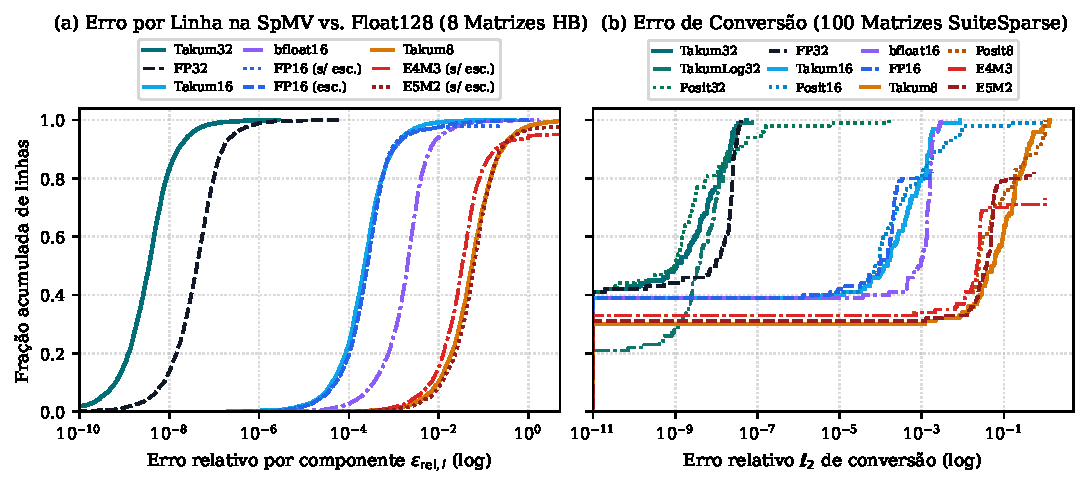
\includegraphics[width=0.66\textwidth]{../paper/figures/error-cdf-pt.pdf}
\end{frame}

\begin{frame}{Resultado 3: Contagem de Instruções, CSRs e Modelo Analítico}
	\begin{itemize}
		\item Modelo exato $N_f = r_f R + c_f S + K$ com \textbf{resíduo máximo \ModResiduoMax} nas \ModExec\ execuções reais e \ModSinteticosOk/\ModSinteticosTotal\ sintéticas ($N_{\text{Takum32}} - N_{\text{FP32}} = R - S \le 0$).
		\item \texttt{Takum32} executa menos (\InsnMenorTrinta) ou igual (\InsnIgualTrinta) instruções em \InsnPares/\InsnPares\ pares, mesmas escritas CSR e reduz elementos ativos de \ElemNnzFP\ para \ElemNnzTakum/nnz ($-15.6\%$).
	\end{itemize}
	\centering
	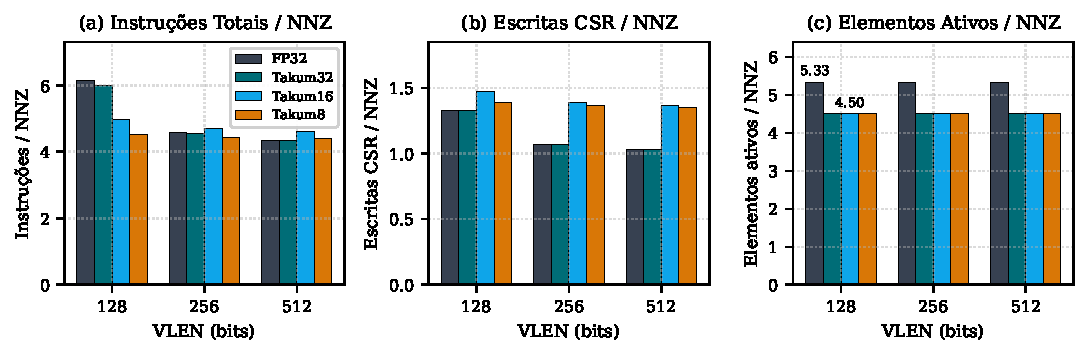
\includegraphics[width=0.82\textwidth]{../paper/figures/insn-csr-comparison-pt.pdf}
\end{frame}

\begin{frame}{Conclusão e Reprodutibilidade (\texttt{scripts/run\_all.py})}
	\begin{itemize}
		\item \textbf{Zvtakum} une janela de 12~MSBs, ULA inteira de 128 bits com RNE no código e cinco instruções em \texttt{custom-0} sem riscos em \texttt{fcsr}.
		\item \texttt{Takum32} reduz o erro mediano em $\RazaoKernelTrinta\times$ frente ao \texttt{FP32} sem nunca exceder instruções; \texttt{Takum8/16} eliminam \emph{overflows} e superam \texttt{bfloat16}.
		\item \textbf{Pipeline único verificável:}
		      \begin{itemize}
		          \item \texttt{python3 scripts/run\_all.py} (ou \texttt{make all-pipeline})
		          \item Executa testes C++/Python, QEMU difftest, 96 kernels SpMV, modelo analítico, baselines numéricos, gráficos e compila \texttt{paper/main.pdf} (EN, 6 pág.), \texttt{paper/main\_pt.pdf} (PT, 6 pág.) e \texttt{slides/slides.pdf}.
		      \end{itemize}
	\end{itemize}
	\vfill
	\centering \large Obrigado! Perguntas?
\end{frame}

\end{document}
